% PREAMBLE
\documentclass[11pt]{amsart}
\usepackage[T1]{fontenc}
\usepackage{lmodern}
\usepackage{microtype}
\usepackage{amsmath,amssymb}
\usepackage{mathtools}
\usepackage{graphicx}
\usepackage{booktabs}
\usepackage{tikz}
\usepackage[colorlinks=true,linkcolor=blue!45!black,citecolor=blue!45!black,urlcolor=blue!45!black]{hyperref}
\usepackage[capitalize]{cleveref}

\newtheorem{theorem}{Theorem}[section]
\newtheorem{proposition}[theorem]{Proposition}
\newtheorem{lemma}[theorem]{Lemma}
\newtheorem{corollary}[theorem]{Corollary}
\newtheorem{conjecture}[theorem]{Conjecture}
\theoremstyle{definition}
\newtheorem{definition}[theorem]{Definition}
\newtheorem{fact}[theorem]{Fact}
\theoremstyle{remark}
\newtheorem{remark}[theorem]{Remark}

\title{The Pincer at Dimension One: Two Edges and Two Closed Doors}
\author{Carlo Mitchener}
\address{MrlyProd, Inc.}
\email{carlo.mitchener@gmail.com}
\date{First published 2026-08-31}

% PAPER
\begin{document}

\begin{abstract}
Take a lattice point of a fractal and ask whether its two coordinates share a common factor; on average the answer is known for every such fractal thicker than a line. Exactly at a line it is open, and what is missing is one estimate about primes of a single size. Writing $\beta = \log_3 p / n$ for the size of a prime $p$ against the level $n$ of the base-$3$ Sierpi\'nski gasket, we pin the troublesome range inside $\beta \in (0.4475978,\allowbreak\, 0.6402121938]$, the upper endpoint being $1/(2 - \log_3 \varphi)$ with $\varphi$ the golden ratio, and proved here; the lower endpoint is the tenth rung of a separate Fourier moment ladder, proved there and imported here. That edge comes from a burst certificate: one combinatorial injection bounding the growth of every one of infinitely many ray automata by $\varphi$, with no computation. Two impossibility results follow, each saying what a new idea must supply.
\end{abstract}

\maketitle

\section{Introduction}
\label{sec:intro}

Pick a level $n$ and build the base-$3$ Sierpi\'nski gasket at that level: the $3^n$ lattice points of the plane whose base-$3$ digit pairs all come from
\[
  F = \{(0,0),\,(1,0),\,(0,1)\}.
\]
Call this set $G_n$. It is the familiar triangle-of-triangles, drawn with integer coordinates instead of ink. Now ask the oldest question in the book: of those $3^n$ points, what fraction has coordinates with greatest common divisor $1$?

\begin{figure}[h]
\centering
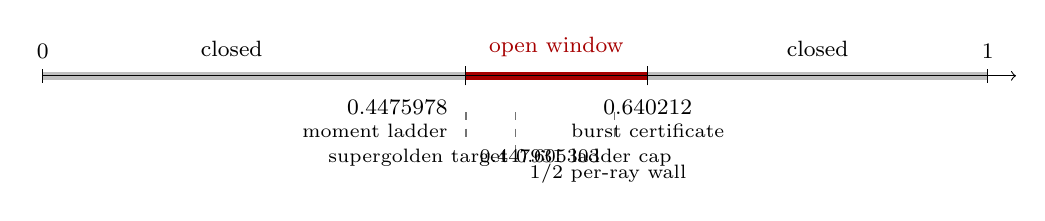
\begin{tikzpicture}[x=12cm,y=1cm]
  \draw[line width=3pt,black!25] (0,0) -- (0.4475978,0);
  \draw[line width=3pt,black!25] (0.640212,0) -- (1,0);
  \draw[line width=3pt,red!65!black] (0.4475978,0) -- (0.640212,0);
  \draw[->] (0,0) -- (1.03,0);
  \foreach \x/\l in {0/0, 1/1} {
    \draw (\x,-0.09) -- (\x,0.09) node[above,font=\footnotesize] {$\l$};
  }
  \draw (0.4475978,-0.12) -- (0.4475978,0.12);
  \draw (0.640212,-0.12) -- (0.640212,0.12);
  \node[font=\footnotesize,align=right,anchor=north east] at ([xshift=-3pt]0.4475978,-0.18) {$0.4475978$\\[-1pt]\scriptsize moment ladder};
  \node[font=\footnotesize,align=center,anchor=north] at (0.640212,-0.18) {$0.640212$\\[-1pt]\scriptsize burst certificate};
  \node[font=\footnotesize,anchor=south] at (0.2,0.12) {closed};
  \node[font=\footnotesize,anchor=south] at (0.82,0.12) {closed};
  \node[font=\footnotesize,red!65!black,anchor=south] at (0.5435,0.12) {open window};
  \draw[dashed,black!55] (0.447931,-0.46) -- (0.447931,-0.86);
  \draw[dashed,black!55] (0.5,-0.46) -- (0.5,-1.06);
  \draw[dashed,black!55] (0.605303,-0.46) -- (0.605303,-0.86);
  \node[font=\scriptsize,anchor=north west] at (0.452,-0.80) {$0.447931$ ladder cap};
  \node[font=\scriptsize,anchor=north west] at (0.505,-1.00) {$1/2$ per-ray wall};
  \node[font=\scriptsize,anchor=north east] at (0.60,-0.80) {supergolden target $0.605303$};
\end{tikzpicture}
\caption{The pincer. Grey is proved closed, red is what remains, and the upper red endpoint is this paper's theorem. The dashed marks are structural walls: no moment order reaches $0.447931$, no per-ray maximum reaches $1/2$. The lower endpoint and the ladder cap are drawn at the same place because they now differ by less than $0.00034$: the ladder is all but spent, and only the upper edge has room to move.}
\label{fig:pincer}
\end{figure}

Above dimension one this is a routine sieve, and the reason is worth seeing, because it is exactly the reason the sieve stops at a line. A prime $p$ in the greatest common divisor confines the point to the sublattice $p\mathbb Z^2$, whose share of a $D$-dimensional digital design is of order $p^{-D}$; summing over the large primes costs $\sum_{p > z} p^{-D}$, which converges for $D > 1$ and can be made small by taking $z$ large. At $D = 1$ that sum is $\sum_{p>z} 1/p$, which diverges for every $z$, and the argument stops. The gasket is the canonical dimension-one object. Nothing below depends on the picture just drawn; it is only the reason dimension one is the interesting case. What blocks the proof there is a single estimate: the points whose coordinates a large prime $p$ divides must not be too many, summed over all large $p$ at once. For a general digital design that estimate is known as \emph{Lemma B}. Only its gasket case is at stake here, and since the two are different statements they get different names: the gasket case is \emph{Lemma G}, written out as \cref{def:lemmag} below.

The estimate is easy for small $p$ and easy for enormous $p$. It is hard in the middle, and ``the middle'' can be named precisely. Write a prime's size against the level as its \emph{exponent}
\[
  \beta = \frac{\log_3 p}{n}.
\]
Two completely different machines close the two ends. From below, a Fourier moment ladder closes every $\beta$ under $0.4475978$; that machine is stated here as \cref{def:hypL} and is not reproduced, because it shares nothing with this paper. From above, and this is what we prove, an elementary automaton argument with no Fourier analysis in it at all closes every $\beta$ above
\[
  \frac{1}{2 - \log_3 \varphi} = 0.6402121938 \dots
\]
Here $\varphi = (1+\sqrt5)/2 = 1.6180339887\ldots$ is the golden ratio \cite{oeisphi}.


\subsection*{Where the upper edge comes from}

Every nonzero point of $G_n$ that is not on an axis is uniquely $g \cdot (a,b)$ with $(a,b)$ a primitive pair. Call $(a,b)$ a \emph{ray}, and call $\max(a,b)$ its \emph{height}. A big prime in the gcd forces a small height, so the top of the range is a counting problem: how many multiples of a short ray can sit inside the gasket?

That count is run by a finite automaton on the base-$3$ digits of $g$, with carry state $(c_1,c_2)$. Its growth rate is the spectral radius $\rho(a,b)$ of the transition matrix, and the whole top range hinges on one bound: $\rho(a,b) \le \varphi$ for \emph{every} ray. The trouble is that there are infinitely many rays and the automaton's size grows like $ab$, so no finite computation settles it.

The burst certificate settles it in one page and with no computation. Each carry state admits $2$, $1$ or $0$ digits, and which one is read off a single residue. The key is a delay: when $3^k$ divides the relevant quantity, the type of a state is fixed $k$ steps in advance, and the two children of a $2$-branching state are forced into \emph{different} types exactly $k$ steps downstream. So a free choice today costs a forced move on day $k$. Record the free choices and you have injected the admissible length-$w$ paths into the subsets of $\{1,\dots,w\}$ with no two elements at distance exactly $k$. Those subsets are counted by a product of Fibonacci numbers, at most $\varphi^{w+k}$, and that is $\rho \le \varphi$ for the entire infinite family at once (\cref{thm:burst}).

\subsection*{Two closed doors}

The edge $0.6402121938$ is not sharp, and we say so loudly. The shift rays $(1,3^k)$ sit exactly at $\varphi$, but no other ray we have ever measured exceeds the supergolden ratio $1.4655712319$, and if that held uniformly the edge would move to $0.6053028664$ (\cref{con:supergolden}). What we prove is narrower and more useful: the two obvious routes to improvement are shut.

\Cref{thm:closure-one} says that keeping the exact Fibonacci product $D_k(w)$ instead of the clean $\varphi^{w+k}$ buys nothing. The depth-one stratum alone, with $j = \lfloor cn \rfloor$, already produces $3^{n\psi_\varphi(c) + o(n)}$ with $\psi_\varphi(c) = 2c + (1-c)\log_3\varphi$, and $\psi_\varphi(c) = 1$ rearranges to exactly $1 - c = 1/(2 - \log_3\varphi)$. This is a statement about the relaxation, not a lower bound for the true ray mass.

\Cref{thm:closure-two} says that averaging the $\rho$'s instead of taking their supremum buys nothing either, and it says so against the strongest version of the temptation. The catalogue really is sub-golden: of the $489$ rays of height at most $40$ under the convention of \cref{fact:catalogue}, all but the three shifts have certified radius below $1.4813$, and the inverse-square-weighted upper mean is $1.0997454$. None of it converts, because ray mass is governed by $\rho^w$ and Jensen's inequality points the wrong way. Any fixed distribution that gives a golden ray positive weight has $w$-th root tending to $\varphi$.

One number must be quarantined here, because it is the punchline. Substituting an averaged radius into $(2 - \log_3\lambda)^{-1}$ produces $0.5145062$ from the inverse-square-weighted mean $1.0639086$, and $0.5226147$ from the certified upper mean $1.0997454$. \emph{Neither is a coprimality bound}, and neither may be quoted as one. They are the output of a substitution that \cref{thm:closure-two} proves invalid.

\subsection*{What is new}

The one-dimensional missing-digit literature is deep and does not reach here. Erd\H{o}s--Mauduit--S\'ark\"ozy \cite{ems}, Konyagin \cite{konyagin} and Maynard \cite{maynard} all prove statements of this shape in one dimension, and all of them operate below these moduli. The decisive obstruction is quantitative: Chow--Varj\'u--Yu \cite{cvy} show in their Remark 6.1 that the Fourier $\ell^1$-dimension of base-$3$ missing-digit measures is provably below $1/2$, so no componentwise transfer from the one-dimensional theory can reach this window. The coupled two-dimensional problem is genuinely new ground rather than an unread special case.

Two ingredients here are classical and are labelled as such, not as contributions. The count $D_k(w)$ of distance-$k$-free subsets factors into Fibonacci numbers because it is the independent-set count on disjoint paths, textbook combinatorics \cite{oeisfib}. And \cref{lem:window}, $\rho(A) \le \|A^w \mathbf 1\|_\infty^{1/w}$ for nonnegative $A$, is the Gelfand row-norm bound. The contribution is \cref{lem:delay} and the injection it powers, the octave census that turns them into an exponent, and the two closures.

\section{Definitions}
\label{sec:defs}

\begin{definition}[The gasket]
\label{def:gasket}
For $n \ge 0$ let $G_n = \bigl\{ \sum_{i<n} d_i 3^i : d_i \in F \bigr\} \subset \mathbb Z^2$ with $F = \{(0,0),(1,0),(0,1)\}$. Then $|G_n| = 3^n$, and the base-$3$ digit expansion of a point of $G_n$ is unique. A point is a \emph{fibre} point if one of its coordinates is $0$; there are $2^{n+1} - 2$ nonzero fibre points, since a point with second coordinate $0$ has all digits in $\{(0,0),(1,0)\}$.
\end{definition}

\begin{definition}[Rays and their automata]
\label{def:ray}
A \emph{ray} is a pair $(a,b)$ of positive integers with $\gcd(a,b) = 1$, taken unordered, since $F$ is symmetric under swapping coordinates. Its \emph{height} is $\max(a,b)$, and it lies in \emph{octave} $j$ when $3^j \le \max(a,b) < 3^{j+1}$. Write $M_n(a,b) = \#\{g \ge 1 : g\,(a,b) \in G_n\}$.

The \emph{ray automaton} of $(a,b)$ has states $(c_1,c_2)$ with $0 \le c_1 < a$ and $0 \le c_2 < b$. A digit $d \in \{0,1,2\}$ is \emph{admissible} at $(c_1,c_2)$ when $\bigl((ad + c_1) \bmod 3,\ (bd + c_2) \bmod 3\bigr) \in F$, and the successor state is $\bigl(\lfloor (ad+c_1)/3 \rfloor,\ \lfloor (bd+c_2)/3 \rfloor\bigr)$. Let $A$ be its $0/1$ transition matrix, $\rho(a,b) = \rho(A)$ its spectral radius, and
\[
  P_w(s) = \bigl(A^w \mathbf 1\bigr)_s
\]
the number of admissible digit paths of length $w$ from state $s$. Reading the base-$3$ digits of $g$ from least significant end, $g\,(a,b) \in G_n$ forces exactly an admissible path from the zero state, so $M_n(a,b) \le \max_s P_{n-j}(s)$ for a ray in octave $j$.
\end{definition}

\begin{definition}[Class and parameter]
\label{def:class}
A ray $(a,b)$ is exactly one of:
\begin{itemize}
  \item \textbf{eq}: $3 \nmid ab$ and $a \equiv b \pmod 3$;
  \item \textbf{opp}: $3 \nmid ab$ and $a \not\equiv b \pmod 3$, so $3 \mid a+b$; set $k = v_3(a+b) \ge 1$;
  \item \textbf{div}: exactly one of $a,b$ is divisible by $3$; write it first, so $3 \mid a$, and set $k = v_3(a) \ge 1$.
\end{itemize}
Coprimality forbids $3 \mid \gcd(a,b)$, so the trichotomy is exhaustive. The \emph{branching type} is $B = 0$ for div and $B = 1$ for opp; $k$ is the \emph{parameter}. The \emph{shift rays} are $(1, 3^k)$ for $k \ge 1$; note that $(1,1)$ is class eq and is \emph{not} a shift.
\end{definition}

\begin{definition}[Distance-free subsets]
\label{def:dk}
For $k, w \ge 1$ let $D_k(w) = \#\{S \subseteq \{1,\dots,w\} : \text{no two elements of } S \text{ differ by exactly } k\}$.
\end{definition}

\begin{definition}[Lemma G and its exponent]
\label{def:lemmag}
Fix a prime $p \ne 3$ and let
\[
  T_p(n) \ = \ \#\{\,x \in G_n \setminus \{0\} \ : \ p \mid \gcd(x_1,x_2)\,\},
\]
the mass a single prime carries in the greatest common divisor. The origin is excluded because it lies in every residue class of every modulus and carries no information. \emph{Lemma G} is the statement
\[
  \lim_{z \to \infty} \ \limsup_{n \to \infty} \ \frac{1}{3^n} \sum_{p > z} T_p(n) \ = \ 0 ,
\]
and \emph{Lemma G holds on an exponent range $I \subseteq (0,1]$} when the same limit taken over the primes with $\log_3 p / n \in I$ is $0$. Both sums are finite: a nonzero point of $G_n$ has both coordinates below $3^n$ and not both zero, so its gcd is a positive integer below $3^n$ and only primes $p < 3^n$ occur at all. The letter keeps this statement apart from Lemma B of the wider coprimality programme, which asserts the same vanishing for a general digital design, with its own point set and its own normalisation; Lemma G is the gasket case and is all that is meant below.
\end{definition}

\begin{definition}[Hypothesis L, the low range]
\label{def:hypL}
\emph{Hypothesis L} is the statement that Lemma G holds on $(0,\ \beta_0]$ for $\beta_0 = 0.447597813453$. It is a theorem of a separate machine, the Fourier moment ladder \cite{ladder}: exact moment identities for the gasket's character sums, a three-block H\"older bound at moment order $2K$ whose middle block is supplied by an energy cap, and a dyadic summation over the primes. Its rungs $\beta_0^{(2K)}$ are indexed by the moment order and rise through the orders computed; the constant above is a truncation of the tenth rung, which is the highest rung whose master bound is written out and whose growth constant is bracketed in exact arithmetic rather than merely computed. It works with the target-uniform count $\max_\tau \#\{x \in G_n : x \equiv \tau \bmod p\}$, which dominates $T_p(n)$, so what it delivers on $(0,\beta_0]$ is at least \cref{def:lemmag}; that weaker consequence is all we import. The argument shares no object with this paper and is not reproduced here, so every statement below that uses it is labelled as using it.

One further statement is imported from the same machine and used nowhere in a proof, only as a signpost: the rungs obey the cap $\beta_0^{(2K)} < 2/(3 + \log_3 5)$ for every $K$, because the Fourier peak forces the ladder parameter $\kappa_{2K}$ below $2$. So no moment order reaches $1/2$, and the tenth rung already sits within $0.00034$ of that cap. Since the cap is far below the upper edge of \cref{thm:topedge}, the ladder can never close the window on its own, however high the moment order: whatever closes it must come from above. The numbers this definition contributes are re-checked arithmetically in \cref{fact:ladder}, and the growth constant behind the tenth rung is re-certified there from scratch.
\end{definition}

\begin{remark}[Scope]
\label{rem:census}
Every statement in this paper is about $G_n$ and about nothing else. The gasket is the canonical dimension-one digital design, and other dimension-one designs are reported to reduce to it; that classification and that reduction are separate work, are not reproduced here, and are not used anywhere below.
\end{remark}

\section{Results}
\label{sec:results}

\begin{theorem}[Burst certificate]
\label{thm:burst}
Let $(a,b)$ be a ray of class div or opp with parameter $k$. Then for every state $s$ and every $w \ge 1$,
\[
  P_w(s) \ \le \ D_k(w) \ = \ \prod_{r=1}^{k} F_{m_r + 2}, \qquad m_r = \#\{ i \in \{1,\dots,w\} : i \equiv r \bmod k \},
\]
where $F_1 = F_2 = 1$; consequently $P_w(s) \le \varphi^{w+k}$ and $\rho(a,b) \le \varphi$. For class eq, $P_w(s) \le 1$ and $\rho(a,b) \le 1$. Hence $\rho(a,b) \le \varphi$ for every ray, at every $3$-adic depth.
\end{theorem}

\begin{theorem}[The upper edge]
\label{thm:topedge}
Write $\psi_\varphi(c) = 2c + (1-c)\log_3\varphi$ and $c = 1 - \beta'$. The number of points of $G_n$ whose two coordinates share a prime factor exceeding $3^{\beta' n}$ satisfies
\[
  N_{\mathrm{top}}(n) \ \le \ 2^{n+1} \ + \ 600 \cdot 3^{\,n\,\psi_\varphi(c)} .
\]
Since $\psi_\varphi(c) < 1$ exactly when $c < c^* = (1 - \log_3\varphi)/(2 - \log_3\varphi) = 0.3597878$, Lemma G holds on $(\beta', 1]$ for every
\[
  \beta' \ > \ 1 - c^* \ = \ \frac{1}{2 - \log_3\varphi} \ = \ 0.6402121938 \dots ,
\]
unconditionally, with no unproved input.
\end{theorem}

\begin{corollary}[The pincer]
\label{cor:pincer}
Under \cref{def:hypL}, Lemma G can fail only for prime exponents in
\[
  \beta \ \in \ (\,0.447597813453,\ \ 0.6402121938\,] .
\]
The upper endpoint is \cref{thm:topedge} and is proved here in full; the lower endpoint is Hypothesis L and is proved elsewhere by the moment ladder, not in this paper. Both endpoints are unconditional; only the labour is divided.
\end{corollary}

\begin{theorem}[Closure one: exact Fibonacci products do not help]
\label{thm:closure-one}
Fix $c \in (0, 1/2)$ and put $j = \lfloor cn \rfloor$, $w = n - j$. Keep the exact bound $P_w(s) \le D_k(w)$ of \cref{thm:burst} in place of $\varphi^{w+k}$ and keep the octave census of \cref{lem:census}. Then the depth-one stratum alone contributes at least $3^{\,n\,\psi_\varphi(c) + O(1)}$ to the resulting bound, where $\psi_\varphi(c) = 2c + (1-c)\log_3\varphi$. Consequently the relaxation cannot certify $N_{\mathrm{top}}(n) = o(3^n)$ for any $c > c^*$, and the threshold it yields is exactly $\beta = 1 - c^* = 1/(2 - \log_3\varphi)$, unchanged.

This is a statement about the relaxation, not a lower bound for the true ray mass.
\end{theorem}

\begin{theorem}[Closure two: averaging the radii does not help]
\label{thm:closure-two}
Let $\nu$ be any probability measure on rays with $\nu(\{r_0\}) = q > 0$ for some ray $r_0$ with $\rho(r_0) = \varphi$; by \cref{lem:shift} every shift ray $(1,3^k)$, $k \ge 1$, is such a ray. Then
\[
  \int \rho^w \, d\nu \ \ge \ \max\Bigl\{ \bigl(\textstyle\int \rho \, d\nu\bigr)^w, \ q\,\varphi^w \Bigr\} ,
\]
and consequently
\[
  \liminf_{w \to \infty} \Bigl( \int \rho^w \, d\nu \Bigr)^{1/w} \ \ge \ \varphi .
\]
Since a ray in octave $j$ carries mass at most $\rho^{\,w}$ with $w = n - j$, and mass is what the octave sum adds, replacing $\sup_r \rho(r)$ by any $\nu$-average leaves the exponent of \cref{thm:topedge} untouched. Moreover the inverse-square weight $1/(a^2+b^2)$ is not a probability measure: $\sum_{(a,b)} 1/(a^2+b^2)$ over rays diverges, so every weighted mean of that shape exists only relative to a height cutoff.
\end{theorem}

\begin{remark}[The quarantined number]
\label{rem:quarantine}
Substituting an averaged radius $\lambda$ into $(2 - \log_3\lambda)^{-1}$, the formula that converts a \emph{uniform} bound into an exponent, gives $0.5145062$ from the inverse-square-weighted mean $\lambda = 1.0639086$ and $0.5226147$ from the certified weighted upper mean $\lambda = 1.0997454$. The first of these two numbers has circulated; it comes from the inverse-square-weighted mean and from nothing else. Neither number is a coprimality bound, and neither may be quoted as one: \cref{thm:closure-two} is precisely the proof that the substitution is invalid. The shifts are not removable by having density zero, either: a zero-density family can still be exponentially numerous and dominate after multiplication by $t^w$. What makes them removable in \cref{thm:topedge} is that their count is $O(1)$ per octave, and even so \cref{thm:topedge} does not remove them, it absorbs them.
\end{remark}

\begin{fact}[Shift saturation]
\label{fact:saturation}
At the zero state, both exactly,
\[
  P_{36}\bigl((9,1)\bigr) = D_2(36) = 45{,}765{,}225, \qquad P_{36}\bigl((27,1)\bigr) = D_3(36) = 53{,}582{,}633 .
\]
So the bound of \cref{thm:burst} is attained and nothing uniform in the ray is sharper. These are the cases $k = 2, 3$ at $w = 36$ of \cref{lem:shift}, which proves the equality for every $k$ and every $w$. Checked by \texttt{scripts/verify.py}.
\end{fact}

\begin{fact}[The height-$40$ catalogue]
\label{fact:catalogue}
There are exactly $490$ unordered primitive rays of height at most $40$. Removing $(1,1)$, which is class eq and not a shift, leaves $489$: the three shifts $(1,3), (1,9), (1,27)$ and $486$ non-shift rays. On the $486$, the certificate $\rho \le \|A^{55}\mathbf 1\|_\infty^{1/55}$ gives largest values $1.4812034260$ at $(4,9)$, then $1.4765525267$ at $(3,10)$ and $1.4728541511$ at $(1,12)$, every one below $\varphi$. Taking the exact value $\varphi$ on the three shifts and that certificate off them, the inverse-square-weighted mean over the $489$ is $1.0997454$. The counts, the certificates and that mean are checked by \texttt{scripts/verify.py} in exact integer arithmetic. The corresponding mean of the \emph{exact} radii is smaller, $1.0639086$, and including $(1,1)$ instead of excluding it moves that one to $1.0481989$; those two numbers are recorded here because the convention must travel with any such mean, and they are outside the script's domain, which certifies rather than diagonalises.
\end{fact}

\begin{fact}[The ladder rungs, and the tenth one certified]
\label{fact:ladder}
With $\kappa = 3 - \log_3 5$ and $\beta_0^{(2K)} = \kappa_{2K} / (2\kappa_{2K} + 2 - \kappa)$, $\kappa_{2K} = 2K - \log_3\lambda_{2K}$:
the order-$8$ growth constant $\lambda_8 = 456 + 3\sqrt{11017}$ gives $\beta_0^{(8)} = 0.446717310462$;
the order-$10$ growth constant $\lambda_{10} = 6664.113662506\ldots$ gives $\beta_0^{(10)} = 0.447597813454\ldots$;
and the cap of \cref{def:hypL} is $2/(3 + \log_3 5) = 0.447930988$.

The tenth rung is the one Hypothesis L uses, and its growth constant is bracketed rather than approximated. Write
\[
  E_{10}(G_a) \ = \ \#\Bigl\{ (x_1,\dots,x_5,\,y_1,\dots,y_5) \in G_a^{10} \ : \ \textstyle\sum_i x_i = \sum_i y_i \Bigr\}
\]
for the tenth additive energy of the gasket. Carrying the digit sums through base $3$ turns this into a walk count on a box $\{-2,\dots,2\}^2$ of carry states, an exact $25 \times 25$ nonnegative integer matrix $M$ with $E_{10}(G_a) = (M^a)_{(0,0),(0,0)}$, so that
\begin{gather*}
  E_{10}(G_a) \ = \ 1,\ 4653,\ 28967859,\ 190911254427, \\
  1270015973323281,\ 8461182216374750493
\end{gather*}
for $a = 0,\dots,5$, the values at $a \le 3$ confirmed independently by direct convolution of the digit set. Its characteristic polynomial factors over $\mathbb Z$ as
\[
  \det(xI - M) \ = \ x^6\,(x-120)\,(x^2-450x+12231)\; c_1(x)^2\, c_2(x)^2\, q(x)
\]
with
\begin{align*}
  c_1(x) &= x^3-2190x^2+282096x-5186835, \\
  c_2(x) &= x^3-990x^2+116154x-2569725, \\
  q(x) &= x^4 - 7833x^3 + 7916949x^2 - 850684437x + 13054946580 .
\end{align*}
The ladder's $\lambda_{10}$ is the Perron root of the strongly connected component of the zero state, a diagonal block of $M$ in strongly connected form, hence one of the real eigenvalues of $M$. A Sturm count in exact rational arithmetic puts no real root of any factor above $66641136626/10^{7}$, and exactly one root of $q$ in the bracket of width $10^{-7}$ immediately below it. Therefore
\[
  \lambda_{10} < 6664.1136626, \quad \kappa_{10} > 1.985805792698, \quad \beta_0^{(10)} > 0.447597813453 ,
\]
every digit truncated down and never rounded up, and the short form $0.4475978$ printed elsewhere in this paper is the same truncation at seven places. Rounding the rung to $0.447598$ would claim a sliver that is not proved, so it is never written that way here.

This Fact asserts the arithmetic, the matrix, the factorisation and the bracket, not the ladder theorems that turn $\lambda_{10}$ into Hypothesis L; those are \cite{ladder}. Everything displayed above is rebuilt from the digit set $F$ and re-checked in exact integer and rational arithmetic by \texttt{scripts/verify.py}, which reads no code of the ladder's.
\end{fact}

\begin{fact}[The census inequalities, verified small]
\label{fact:census}
For every octave $1 \le j \le 4$ and every parameter $k \ge 1$, direct enumeration of all primitive pairs confirms the three upper bounds of \cref{lem:census}, namely at most $9 \cdot 3^{2j-k}$ div rays, at most $18 \cdot 3^{2j-k}$ opp rays and at most $9 \cdot 3^{2j}$ eq rays, and confirms the depth-one count against the stronger threshold $3^{2j-1}$, rather than the $3^{2j-2}$ that \cref{lem:census} proves for large $j$. Checked by \texttt{scripts/verify.py}.
\end{fact}

\begin{conjecture}[Strictness and the supergolden supremum]
\label{con:supergolden}
$\rho(a,b) < \varphi$ for every non-shift ray, with $\sup \rho = 1.4655712319$, the real root of $x^3 = x^2 + 1$ \cite{oeissuper}. Under it, \cref{thm:topedge} improves to every $\beta'$ above $1/(2 - \log_3 1.4655712319)$, that is above $0.6053028664$.

\emph{Evidence.} All $1{,}102$ coprime rays of height at most $60$ were generated and their radii computed independently: $(4,9)$, $(3,10)$ and $(1,12)$ all sit at $1.465571231876768$, the supergolden root to numerical precision; the next family, at $(3,7)$, sits at $1.380277569$; nothing off the shifts approaches $\varphi$. Every radius observed is a root of $x^m = x^{m-1} + 1$ or $x^m = x + 1$, exactly the run-length-constrained counts that near-shift geometry predicts. The certified upper bounds of \cref{fact:catalogue} confirm this at height $40$ with exact integer arithmetic. A mechanism is visible in \cref{thm:burst}: the deep carry $\lfloor c_1 / 3^k \rfloor$ is a deterministic function of the state, and the shifts are exactly the rays where it always sits where the adversary would put it.

\emph{Failure mode.} A finite height box cannot prove a supremum, and the state space grows with $ab$, so the certificate is not uniform. The conjecture dies if some family of non-shift rays of growing height has $\rho \to \varphi$; nothing in the height-$60$ data rules that out, since every observed spectrum is a root of a run-length polynomial and those roots do accumulate at $\varphi$ as the run length grows. An early apparent excess above supergolden in a coarse finite-length estimator was prefactor bias and vanished under exact eigenvalues, which is a warning about how this conjecture will be tested.
\end{conjecture}

\begin{conjecture}[Statement (A), the averaged theorem that would work]
\label{con:statementA}
There are $C > 0$, a polynomial factor, and $\lambda < \varphi$ such that for every octave $j$,
\[
  \sum_{\substack{(a,b) \text{ primitive non-shift} \\ 3^j \le \max(a,b) < 3^{j+1}}} M_n(a,b) \ \le \ C\, 3^{2j}\, \lambda^{\,n-j}\, \mathrm{poly}(n) .
\]
Inserted into the octave sum of \cref{thm:topedge}, it moves the edge to $1/(2 - \log_3\lambda)$. The equivalent tail form asks that the octave-$j$ count of rays with $\rho \ge t$ be at most $3^{2j - I(t)j + o(j)}$, followed by an optimisation over $t$.

\emph{Evidence.} It is weaker than a uniform non-shift spectral gap and far stronger than any average of $\rho$, and \cref{fact:catalogue} is consistent with it: the finite constant $1/(2 - \log_3 1.4812034260) = 0.6088620819$ is what height $40$ would give if the certificate were uniform.

\emph{Failure mode and named obstructions.} It is not uniform, since the state space grows with $ab$, so the finite scan is evidence and not an improvement. Two routes are named and neither is complete: a large sieve applied to a bounded local deficit observable, Fourier-expanded over the ray's residue modulus, and a finite-state fractional-moment operator. One route is explicitly ruled out: Tur\'an power sums detect extremal eigenvalues and lower-bound maxima, whereas this needs an upper bound for a positive sum over many nonnegative matrices of varying dimension, with no cancellation to exploit.
\end{conjecture}

\begin{conjecture}[The second-moment route]
\label{con:z}
A second moment over ray pairs, $Z(n) = \sum_y M_n(y)^2$, is conjectured to satisfy $Z(n) = 2 \cdot 3^n + o(3^n)$; under it the window of \cref{cor:pincer} shrinks to $(0.447597813453,\ 1/2]$, and the per-ray wall at $1/2$ of \cref{fig:pincer} is then the binding one.

\emph{Evidence.} $Z(n)$ decomposes exactly into an arithmetic part with closed form plus a residual, and the arithmetic part already carries the constant $2$; the residual is measured to $n = 18$ and decays.

\emph{Failure mode.} The single remaining step is that the residual is $o(3^n)$, which is not proved. A reading in which the residual grows like $\varphi^{2n}$ is refuted by the same data, whose measured decay ratio near $n = 18$ is about $2.52$, below $\varphi^2 = 2.618$; so the residual is not governed by $\varphi^2$ and the conjecture waits on a genuine estimate rather than on an extrapolated ratio.
\end{conjecture}

\section{Proofs}
\label{sec:proofs}

\begin{lemma}[Window lemma; classical]
\label{lem:window}
For a nonnegative square matrix $A$ and every $w \ge 1$, $\rho(A) \le \bigl(\max_s (A^w \mathbf 1)_s\bigr)^{1/w}$.
\end{lemma}

\begin{proof}
$\rho(A)^w = \rho(A^w) \le \|A^w\|_\infty$, since the spectral radius is at most any induced norm. For a nonnegative matrix the induced $\infty$-norm is the maximal row sum, which is $\max_s (A^w \mathbf 1)_s$. Take $w$-th roots.
\end{proof}

\begin{lemma}[Branching types]
\label{lem:types}
Let $(a,b)$ be a ray and $(c_1,c_2)$ a state of its automaton.
\begin{enumerate}
  \item \emph{div}, $3 \mid a$, $3 \nmid b$: the first output residue $t = (ad+c_1) \bmod 3 = c_1 \bmod 3$ is digit-independent. If $t = 2$ there are $0$ admissible digits; if $t = 1$ there is exactly $1$; if $t = 0$ there are exactly $2$, and they are distinct residues mod $3$.
  \item \emph{opp}, $3 \mid a+b$, $3 \nmid ab$: the residue sum $s = (r_1 + r_2) \bmod 3 = (c_1+c_2) \bmod 3$ is digit-independent. If $s = 2$ there are $0$ admissible digits; if $s = 0$ there is exactly $1$; if $s = 1$ there are exactly $2$, distinct mod $3$.
  \item \emph{eq}, $3 \nmid ab$, $a \equiv b$: there is at most $1$ admissible digit.
\end{enumerate}
\end{lemma}

\begin{proof}
(1) $ad \equiv 0$, so $t = c_1 \bmod 3$ does not depend on $d$. No element of $F$ has first coordinate $2$, so $t = 2$ kills the state. If $t = 1$, the only element of $F$ with first coordinate $1$ is $(1,0)$, so $d$ must satisfy $bd \equiv -c_2 \pmod 3$; since $3 \nmid b$ the map $d \mapsto bd$ is a bijection mod $3$ and exactly one $d$ qualifies. If $t = 0$, the elements $(0,0)$ and $(0,1)$ are available, requiring $bd \equiv -c_2$ and $bd \equiv 1-c_2$ respectively; each has exactly one solution and the two solutions differ.

(2) $r_1 + r_2 \equiv (a+b)d + c_1 + c_2 \equiv c_1 + c_2 = s$, again digit-independent. The elements of $F$ have coordinate sums $0, 1, 1$, so $s = 2$ kills the state. If $s = 0$ only $(0,0)$ is possible: $ad \equiv -c_1$ has exactly one solution since $3 \nmid a$, and then $r_2 \equiv s - r_1 \equiv 0$ automatically. If $s = 1$ then $(1,0)$ and $(0,1)$ are possible, requiring $ad \equiv 1-c_1$ and $ad \equiv -c_1$; each has one solution and the two differ.

(3) $r_1 - r_2 \equiv (a-b)d + c_1 - c_2 \equiv c_1 - c_2$ is digit-independent. The elements of $F$ have coordinate differences $0, 1, -1$, so at most one element of $F$ is reachable, and it pins $r_1$; since $3 \nmid a$ the map $d \mapsto (ad + c_1) \bmod 3$ is a bijection, so at most one $d$ qualifies.
\end{proof}

\begin{lemma}[Delayed split]
\label{lem:delay}
Let $(a,b)$ be of class div or opp with parameter $k$ and branching type $B$. Fix a state at step $i$ and an admissible continuation. Then:
\begin{enumerate}
  \item for $1 \le j < k$, the type at step $i+j$ is determined by the state at step $i$ alone;
  \item the type at step $i+k$ is determined by the state at step $i$ together with the single digit $d_i$, and the two admissible digits at a $2$-branching step give \emph{distinct} types at step $i+k$.
\end{enumerate}
\end{lemma}

\begin{proof}
\emph{div.} Write $a = 3^k a'$ with $3 \nmid a'$. Since $ad = 3^k a' d$ we have exactly
\[
  c_1^{(i+1)} = \Bigl\lfloor \frac{a d_i + c_1^{(i)}}{3} \Bigr\rfloor = 3^{k-1} a' d_i + \Bigl\lfloor \frac{c_1^{(i)}}{3} \Bigr\rfloor .
\]
We claim, for $0 \le j \le k$,
\[
  c_1^{(i+j)} = a' \sum_{m < j} 3^{\,k-j+m}\, d_{i+m} \ + \ \Bigl\lfloor \frac{c_1^{(i)}}{3^{\,j}} \Bigr\rfloor .
\]
The case $j = 1$ is the displayed recursion. Assume it for some $j < k$. Every exponent $k-j+m$ with $0 \le m < j$ is at least $k - j \ge 1$, so each term of the sum is divisible by $3$, and applying the recursion once more,
\begin{align*}
  c_1^{(i+j+1)} &= 3^{k-1}a' d_{i+j} + \Bigl\lfloor \frac{c_1^{(i+j)}}{3} \Bigr\rfloor \\
   &= 3^{k-1} a' d_{i+j} + a' \sum_{m<j} 3^{\,k-j-1+m} d_{i+m} + \Bigl\lfloor \frac{c_1^{(i)}}{3^{\,j+1}} \Bigr\rfloor ,
\end{align*}
which is the claim at $j+1$ because $3^{k-1} = 3^{\,k-(j+1)+j}$. Now the type at step $i+j$ is $t_{i+j} = c_1^{(i+j)} \bmod 3$ by \cref{lem:types}. For $j < k$ every exponent $k-j+m \ge 1$, so the digit terms vanish mod $3$ and $t_{i+j} \equiv \lfloor c_1^{(i)}/3^{\,j} \rfloor$, which is (1). At $j = k$ the exponents are $m$ for $0 \le m < k$, so only $m = 0$ survives mod $3$:
\[
  t_{i+k} \ \equiv \ a' d_i + \Bigl\lfloor \frac{c_1^{(i)}}{3^{\,k}} \Bigr\rfloor \pmod 3 .
\]
At a $2$-branching state the two admissible digits are distinct mod $3$ by \cref{lem:types}, and $3 \nmid a'$, so $a'd_i$ separates them, and the two types at step $i+k$ differ. That is (2).

\emph{opp.} Write $a + b = 3^k m$ with $3 \nmid m$, and $T_i = c_1^{(i)} + c_2^{(i)}$. On an admissible step with output $(r_1,r_2) \in F$,
\[
  T_{i+1} = \frac{(a+b)d_i + T_i - \varrho_i}{3} = 3^{k-1} m\, d_i + \frac{T_i - \varrho_i}{3}, \qquad \varrho_i = r_1 + r_2 \in \{0,1\} ,
\]
and by \cref{lem:types} $\varrho_i$ is determined by $T_i \bmod 3$ alone ($\varrho = 0$ when $s = 0$, $\varrho = 1$ when $s = 1$, and $s = 2$ is dead), with $T_i - \varrho_i \equiv 0 \bmod 3$. Define $N_0 = T_i$ and $N_{j+1} = (N_j - \varrho(N_j \bmod 3))/3$. Exactly as above one proves, for $0 \le j \le k$,
\[
  T_{i+j} = m \sum_{m' < j} 3^{\,k-j+m'} d_{i+m'} \ + \ N_j ,
\]
the induction being legitimate because for $j < k$ the digit terms are divisible by $3$, hence $T_{i+j} \equiv N_j \bmod 3$ and the subtracted $\varrho$ is the one the recursion for $N_j$ uses. Therefore $s_{i+j} = N_j \bmod 3$ for $j < k$, which is (1), and $s_{i+k} \equiv m d_i + N_k \bmod 3$, which separates the two admissible digits since $3 \nmid m$. That is (2).
\end{proof}

\begin{lemma}[Distance-free subsets; classical]
\label{lem:subsets}
$D_k(w) = \prod_{r=1}^{k} F_{m_r+2}$ with $m_r = \#\{i \le w : i \equiv r \bmod k\}$, and $\varphi^{\,w} \le D_k(w) \le \varphi^{\,w+k}$.
\end{lemma}

\begin{proof}
Partition $\{1,\dots,w\}$ into the $k$ residue chains modulo $k$. Two elements differ by exactly $k$ if and only if they are consecutive within one chain, so an admissible $S$ is exactly a choice of an independent set in each of $k$ disjoint paths, of lengths $m_1,\dots,m_k$ summing to $w$. Independent sets in a path on $m$ vertices number $F_{m+2}$, the standard recursion. For the upper bound, $F_{m+2} \le \varphi^{\,m+1}$ holds for $m = 0, 1$ and propagates: $F_{m+2} = F_{m+1} + F_m \le \varphi^{\,m} + \varphi^{\,m-1} = \varphi^{\,m-1}(\varphi+1) = \varphi^{\,m+1}$. Multiplying over the chains gives $\prod \varphi^{\,m_r+1} = \varphi^{\,w+k}$. For the lower bound, $F_{m+2} \ge \varphi^{\,m}$ holds for $m = 0,1$ and propagates the same way, $F_{m+2} = F_{m+1}+F_m \ge \varphi^{\,m-1}+\varphi^{\,m-2} = \varphi^{\,m}$; multiplying over the chains gives $\varphi^{\sum_r m_r} = \varphi^{\,w}$.
\end{proof}

\begin{proof}[Proof of \cref{thm:burst}]
Class eq is immediate from \cref{lem:types}(3): at most one admissible digit at every state gives $P_w(s) \le 1$ and, by \cref{lem:window}, $\rho \le 1$.

Let $(a,b)$ be div or opp with parameter $k$ and branching type $B$. At each $2$-branching state, \cref{lem:delay}(2) gives the two admissible digits distinct types at step $i+k$, so at most one of those two types equals $B$. Define the \emph{designated} digit at a $2$-branching step $i$ to be the admissible digit whose type at step $i+k$ is not $B$, choosing the smaller digit when both qualify, and choosing the smaller digit also when the predetermined window ahead is dead, meaning one of the types $t_{i+1},\dots,t_{i+k-1}$ fixed by \cref{lem:delay}(1) equals $2$. The rule is total, and in the dead-window case the designation is never consulted, because no admissible path of the length under consideration passes through step $i+k$.

Fix a start state $s$ and $w \ge 1$. To an admissible path $(d_0,\dots,d_{w-1})$ assign the subset $S \subseteq \{1,\dots,w\}$ given by
\[
  S \ = \ \bigl\{\, i + 1 \ : \ 0 \le i < w, \ \text{step } i \text{ is } 2\text{-branching},
  \ d_i \text{ designated} \,\bigr\} .
\]

\emph{The map is injective.} Two distinct admissible paths from $s$ agree up to some first index $i$ and differ there. Both continuations being admissible, step $i$ has two admissible digits, so it is $2$-branching by \cref{lem:types}, and the states along the two paths coincide up to step $i$, so both paths see the same designation there. Exactly one of the two digits is designated, so $i+1$ lies in one image set and not the other.

\emph{The image avoids distance $k$.} Suppose $i+1 \in S$ and $i+1+k \le w$. Then $d_i$ is designated, and the window $t_{i+1},\dots,t_{i+k-1}$ is alive, since the path is admissible through step $i+k$. Hence the designation was made by the type rule and the type at step $i+k$ is not $B$. By \cref{lem:types}, only type-$B$ steps are $2$-branching, so step $i+k$ is not $2$-branching and $i+1+k \notin S$.

Therefore $P_w(s) \le D_k(w)$, and \cref{lem:subsets} gives $P_w(s) \le \varphi^{\,w+k}$. Finally \cref{lem:window} applied at every $w$ gives $\rho(a,b) \le (\varphi^{\,w+k})^{1/w} \to \varphi$, so $\rho(a,b) \le \varphi$.
\end{proof}

\begin{lemma}[The shift rays are exactly golden]
\label{lem:shift}
Let $k \ge 1$ and take the shift ray $(1,3^k)$, written with its $3$-divisible coordinate first as $(a,b) = (3^k,1)$. Then $P_w(0) = D_k(w)$ at the zero state for every $w \ge 1$, and $\rho(1,3^k) = \varphi$.
\end{lemma}

\begin{proof}
Since $b = 1$ the second carry is always $0$, so a state is a single integer $c$ with $0 \le c < 3^k$. On a digit $d$ the output residues are $r_1 = (3^k d + c) \bmod 3 = c \bmod 3$ and $r_2 = d \bmod 3 = d$, and the successor is
\[
  c \ \longmapsto \ \Bigl\lfloor \frac{3^k d + c}{3} \Bigr\rfloor \ = \ 3^{\,k-1} d + \Bigl\lfloor \frac{c}{3} \Bigr\rfloor .
\]
The ray is class div with parameter $k$, so by \cref{lem:types}(1) the state $c$ is $2$-branching when $c \equiv 0$, where the two admissible digits are $d = 0$ and $d = 1$, producing the outputs $(0,0)$ and $(0,1)$; it admits the single digit $d = 0$ when $c \equiv 1$, producing $(1,0)$; and it is dead when $c \equiv 2$.

Start at $c_0 = 0$. We claim
\[
  c_i \ = \ \sum_{j=1}^{\min(i,k)} 3^{\,k-j}\, d_{i-j} .
\]
This is trivial at $i = 0$. Assume it at $i$. Every term with $j < k$ is divisible by $3$, and the term $j = k$, which is present only when $i \ge k$, equals $d_{i-k} < 3$. Hence $\lfloor c_i/3 \rfloor = \sum_{j=1}^{\min(i,\,k-1)} 3^{\,k-1-j} d_{i-j}$, and since $\min(i,k-1) + 1 = \min(i+1,k)$, reindexing turns $c_{i+1} = 3^{\,k-1} d_i + \lfloor c_i/3\rfloor$ into the claim at $i+1$. Reducing modulo $3$, only the $j = k$ term survives:
\[
  c_i \equiv 0 \pmod 3 \quad (i < k), \qquad c_i \equiv d_{\,i-k} \pmod 3 \quad (i \ge k).
\]
Every admissible digit is $0$ or $1$, so $c_i \bmod 3$ is never $2$: no state on a path from the zero state is dead. Consequently an admissible path of length $w$ from the zero state is exactly a string $(d_0,\dots,d_{w-1}) \in \{0,1\}^w$ in which $d_i = 1$ forces $d_{i+k} = 0$ whenever $i + k < w$, and $d_i = 0$ leaves $d_{i+k}$ free. Sending the path to $\{\,i+1 : d_i = 1\,\}$ is a bijection onto the subsets of $\{1,\dots,w\}$ with no two elements at distance exactly $k$, so $P_w(0) = D_k(w)$.

By \cref{lem:subsets}, $D_k(w) \ge \varphi^{\,w}$, so $P_w(0) \ge \varphi^{\,w}$. Since $P_w(0) \le \|A^w\|_\infty$ and $\rho(A) = \lim_{w} \|A^w\|_\infty^{1/w}$ by Gelfand's formula, this gives $\rho \ge \varphi$, and \cref{thm:burst} gives $\rho \le \varphi$.
\end{proof}

\begin{lemma}[Octave census]
\label{lem:census}
Fix an octave $j \ge 1$ and a parameter $k \ge 1$. Among primitive pairs of height in $[3^j, 3^{j+1})$ there are at most $9 \cdot 3^{2j-k}$ of class div with $v_3(a) = k$, at most $18 \cdot 3^{2j-k}$ of class opp with $v_3(a+b) = k$, and at most $9 \cdot 3^{2j}$ of class eq. Moreover the div class has parameter $k \le j$ and the opp class $k \le j+1$. Finally, for all large $j$ the number of div rays with $k = 1$ is at least $3^{2j-2}$.
\end{lemma}

\begin{proof}
Both coordinates are less than $3^{j+1}$. For div we may name the $3$-divisible coordinate $a$, since the pair is unordered; then $3^k \mid a$ and $a < 3^{j+1}$ leave at most $3^{\,j+1-k}$ choices of $a$ and fewer than $3^{\,j+1}$ of $b$, giving at most $3^{\,2j+2-k} = 9 \cdot 3^{2j-k}$ pairs, and $3^k \le a < 3^{j+1}$ forces $k \le j$. For opp, choose $a$ freely among fewer than $3^{\,j+1}$ values; then $b \equiv -a \bmod 3^k$ with $b < 3^{j+1}$ leaves at most $3^{\,j+1-k} + 1 \le 2 \cdot 3^{\,j+1-k}$ values, giving at most $2 \cdot 3^{\,2j+2-k} = 18 \cdot 3^{2j-k}$, and $3^k \le a+b < 2 \cdot 3^{j+1}$ forces $k \le j+1$. For eq, both coordinates are free below $3^{j+1}$, giving at most $9 \cdot 3^{2j}$.

For the lower bound put $N = 3^j$ and count pairs $(a,b)$ with $a = 3a'$, $a' \in [N/3, N)$, $3 \nmid a'$, $b \in [1, 3N)$, $3 \nmid b$, $\gcd(a', b) = 1$. Every such pair is primitive with $v_3(a) = 1$ and height $a \in [N, 3N)$, so it is a div ray with $k = 1$ in octave $j$, and distinct pairs give distinct rays. The number of admissible $a'$ is $\tfrac23 \cdot \tfrac{2N}{3} + O(1) = \tfrac{4N}{9} + O(1)$ and of admissible $b$ is $2N + O(1)$, so the box holds $\tfrac{8}{9}N^2 + O(N)$ pairs. By Bonferroni, discarding only the first-order terms of inclusion--exclusion is a valid lower bound, so it suffices to subtract, for each prime $p \ne 3$, the pairs with $p \mid a'$ and $p \mid b$; these number at most $(\tfrac{2N}{3p}+1)(\tfrac{3N}{p}+1) \le \tfrac{2N^2}{p^2} + O(N/p)$. Since $\sum_p p^{-2} = 0.4522\ldots$, removing $p = 3$ leaves $\sum_{p \ne 3} p^{-2} < 0.3412$, so the subtraction is at most $0.6824\,N^2 + O(N\log N)$. The count is therefore at least $(\tfrac89 - 0.6824)N^2 + O(N \log N) > 0.2\,N^2$ for large $j$. Since $0.2 > \tfrac19$, that exceeds $N^2/9 = 3^{2j-2}$ once $N$ is large.
\end{proof}

\begin{proof}[Proof of \cref{thm:topedge}]
Let $x \in G_n$ be nonzero with a prime $p > 3^{\beta' n}$ dividing both coordinates. If $x$ is a fibre point it is one of the $2^{n+1}-2$ of \cref{def:gasket}. Otherwise write $x = g\,(a,b)$ with $(a,b)$ primitive and $g = \gcd(x_1,x_2)$, so $p \mid g$ and $g > 3^{\beta' n}$. Both coordinates of $x$ are below $3^n$, so the height satisfies $\max(a,b) < 3^{n}/g < 3^{(1-\beta')n}$, that is, the octave obeys $j \le cn$ with $c = 1-\beta'$. Hence
\[
  N_{\mathrm{top}}(n) \ \le \ 2^{n+1} \ + \ \sum_{j \le cn} \ \sum_{\substack{(a,b) \text{ primitive} \\ \text{octave } j}} M_n(a,b) .
\]
By \cref{def:ray}, $M_n(a,b) \le \max_s P_{n-j}(s)$. Put $w = n-j$. By \cref{thm:burst}, a class-eq ray contributes at most $1$ and a div or opp ray with parameter $k$ contributes at most $\varphi^{\,w+k}$. Using \cref{lem:census} the octave-$j$ inner sum is at most
\[
  9 \cdot 3^{2j} \ + \ \sum_{k \ge 1} \bigl(9 + 18\bigr) 3^{2j-k} \varphi^{\,w+k}
  \ = \ 9 \cdot 3^{2j} \ + \ 27 \cdot 3^{2j} \varphi^{\,w} \sum_{k \ge 1} \Bigl(\frac{\varphi}{3}\Bigr)^{k} ,
\]
and the geometric series converges because parameter rarity $3^{-k}$ beats mass growth $\varphi^{k}$: its value is $(\varphi/3)/(1-\varphi/3) = 1.1709\ldots$, so the inner sum is at most $9 \cdot 3^{2j} + 31.7 \cdot 3^{2j}\varphi^{\,n-j}$. Summing over octaves, $\sum_{j \le cn} 3^{2j} \le \tfrac98 \, 3^{2cn}$ and
\[
  \sum_{j \le cn} 3^{2j} \varphi^{\,n-j} = \varphi^{\,n} \sum_{j \le cn} (9/\varphi)^{\,j}
  \ \le \ \frac{\varphi^{n}}{1 - \varphi/9} \, (9/\varphi)^{cn}
  \ \le \ 1.22 \cdot \varphi^{\,(1-c)n} 9^{\,cn} ,
\]
which is $1.22 \cdot 3^{\,n \psi_\varphi(c)}$,
since $9^{cn}\varphi^{(1-c)n} = 3^{\,n(2c + (1-c)\log_3\varphi)}$. As $2c \le \psi_\varphi(c)$, the first piece is absorbed, and
\[
  N_{\mathrm{top}}(n) \ \le \ 2^{n+1} + \bigl(10.2 + 38.7\bigr) 3^{\,n\psi_\varphi(c)} \ \le \ 2^{n+1} + 600 \cdot 3^{\,n\psi_\varphi(c)} ,
\]
with the stated constant left generous. Writing $L = \log_3\varphi$, $\psi_\varphi(c) < 1$ is $c(2-L) < 1-L$, that is $c < c^* = (1-L)/(2-L)$, and $1 - c^* = 1/(2-L)$. So for every $\beta' > 1/(2-L)$ we get $N_{\mathrm{top}}(n) = o(3^n)$, since $2^{n+1} = o(3^n)$ as well.

Finally, Lemma G on $(\beta',1]$ follows. Let $p$ be a prime with $\log_3 p / n \in (\beta',1]$, so $p > 3^{\beta' n}$. Every point counted by $T_p(n)$ of \cref{def:lemmag} is a nonzero point of $G_n$ whose gcd is divisible by such a prime, hence is one of the $N_{\mathrm{top}}(n)$ points just bounded. A single point is counted for at most $1/\beta'$ of these primes, since their product divides its gcd and that is below $3^n$. Therefore
\[
  \sum_{\log_3 p / n \, \in \, (\beta',\,1]} T_p(n) \ \le \ \frac{1}{\beta'}\, N_{\mathrm{top}}(n) \ = \ o(3^n) ,
\]
so the inner $\limsup$ of \cref{def:lemmag} restricted to this range is $0$ for every $z$, and so is the limit.
\end{proof}

\begin{proof}[Proof of \cref{thm:closure-one}]
The relaxation in question is the bound of the previous proof with $\varphi^{\,w+k}$ replaced by the exact $D_k(w)$ of \cref{thm:burst}, the octave census of \cref{lem:census} left in place. Its value is a sum of nonnegative terms, so it is at least its depth-one stratum, namely the number of octave-$j$ div rays with $k=1$ times the value of $D_1(w)$ available to them, and $D_1(w) \ge \varphi^{\,w}$ by \cref{lem:subsets}. By the last clause of \cref{lem:census} the stratum has at least $3^{2j-2}$ members for large $j$, so with $j = \lfloor cn \rfloor$ and $w = n-j$ the stratum contributes at least
\[
  3^{2j-2}\, \varphi^{\,n-j} \ = \ 3^{\,-2}\,3^{\,n(2c + (1-c)\log_3\varphi) + O(1)} \ = \ 3^{\,n \psi_\varphi(c) + O(1)} .
\]
A bound of value at least $3^{\,n\psi_\varphi(c)+O(1)}$ certifies $o(3^n)$ only if $\psi_\varphi(c) < 1$, that is only if $c < c^*$. Solving $\psi_\varphi(c) = 1$ gives $c = c^*$ and $\beta = 1 - c^* = 1/(2 - \log_3\varphi)$, the same threshold \cref{thm:topedge} already reaches. So the exact Fibonacci product changes constants and subexponential factors and nothing else.

We repeat the caveat, because it is easy to misread this theorem as a lower bound on ray mass: it is a statement about the relaxation. The true mass of the depth-one stratum may well be far smaller; what is proved is that this particular chain of inequalities cannot see that.
\end{proof}

\begin{proof}[Proof of \cref{thm:closure-two}]
The first inequality is Jensen applied to the convex function $t \mapsto t^w$ on $[0,\infty)$; the second is monotonicity, since $\int \rho^w d\nu \ge \nu(\{r_0\})\rho(r_0)^w = q\varphi^w$. Taking $w$-th roots gives $(\int\rho^w d\nu)^{1/w} \ge q^{1/w}\varphi$, which tends to $\varphi$. The shift rays do have $\rho = \varphi$, for every $k \ge 1$, by \cref{lem:shift}.

For the consequence, note that the octave-$j$ inner sum of the proof of \cref{thm:topedge} is a sum of ray masses, each at most $\rho^{\,w}$ up to the parameter factor, with $w = n-j$. Any scheme that replaces the supremum of $\rho$ over the octave by a $\nu$-average of $\rho$ is asserting $\int \rho^w d\nu \le (\int \rho\, d\nu)^w$, the reverse of the first inequality. Since some rays in every octave large enough to contain one are shifts, $q > 0$ for the natural choices of $\nu$, and the $w$-th root of the true quantity tends to $\varphi$. So the exponent $\psi_\varphi$ is unchanged.

For the last clause, let $H \ge 2$. For each prime $m \le H$ the pairs $(a,m)$ with $1 \le a < m$ are primitive, number $m - 1 \ge m/2$, and satisfy $a^2 + m^2 \le 2m^2$. Hence
\[
  \sum_{\substack{(a,b) \text{ primitive} \\ \max(a,b) \le H}} \frac{1}{a^2+b^2} \ \ge \ \sum_{\substack{m \le H \\ m \text{ prime}}} \frac{m/2}{2m^2} \ = \ \frac14 \sum_{m \le H,\ m \text{ prime}} \frac1m ,
\]
which tends to infinity with $H$ by Mertens \cite{mertens}. So the inverse-square weight has infinite total mass on rays and is a probability measure only after a height cutoff; every mean computed from it, including the two in \cref{rem:quarantine}, is a statement about a particular cutoff and not about rays.
\end{proof}

\begin{proof}[Proof of \cref{cor:pincer}]
\Cref{thm:topedge} gives Lemma G on $(\beta',1]$ for every $\beta' > 0.6402121938$, hence on $(0.6402121938, 1]$ by taking a decreasing sequence of such $\beta'$ and noting that the exponent ranges nest. \Cref{def:hypL} gives it on $(0, 0.447597813453]$. The union leaves exactly the stated interval, on which nothing is claimed.
\end{proof}

\section{Reproducibility}
\label{sec:repro}

One script, \texttt{scripts/verify.py}, re-checks everything numerical in this paper. It uses the Python standard library only, takes no arguments, reads no files, and runs from the lane root in a couple of seconds on a laptop. Every assertion in it names the value obtained and the value expected, and any mismatch aborts the run. It covers exactly the following.

\begin{itemize}
  \item \emph{Constants.} The value $\log_3\varphi$, the edge $1/(2-\log_3\varphi) = 0.6402121938$ that it gives, and the exponent $c^* = 0.3597878$ behind that edge. Then the supergolden root $1.4655712319$, with the edge $0.6053028664$ that it would give in turn, and the ladder cap $2/(3+\log_3 5) = 0.447930988$. Then the two rungs of \cref{fact:ladder}: $0.446717310462$ from $\lambda_8 = 456+3\sqrt{11017}$ and $0.447597813454$ from $\lambda_{10} = 6664.113662506$.
  \item \emph{\cref{fact:ladder}, the tenth rung, from scratch.} The order-$10$ carry matrix rebuilt from $F$ alone on the box $\{-2,\dots,2\}^2$, its six energies $E_{10}(G_a)$ for $a \le 5$, the values at $a \le 3$ against direct convolution of the digit set, the degree-$25$ characteristic polynomial in exact rational arithmetic against the displayed factorisation, and Sturm chains over $\mathbb Q$ placing no real root of any factor above the exact rational $6664.1136626$, with exactly one root of $q$ in the bracket below it, whence the truncated bounds $\kappa_{10} > 1.985805792698$ and $\beta_0^{(10)} > 0.447597813453$. The closure $\lfloor (r+K)/3 \rfloor \le r$ of the carry box and the order-$4$ control $E_4(G_a) = 15^a$ are checked alongside.
  \item \emph{The quarantined substitutions of \cref{rem:quarantine}.} The two identities
  \[
    1/(2-\log_3 1.0639086) = 0.5145062, \qquad 1/(2-\log_3 1.0997454) = 0.5226147 ,
  \]
  checked as arithmetic so that the two numbers are never confused.
  \item \emph{\cref{lem:subsets}.} $D_k(w)$ against brute-force enumeration of all subsets, for $w \le 14$ and $1 \le k \le 5$; and the bound $D_k(w) \le \varphi^{\,w+k}$ for $1 \le k \le 6$ and $w \le 60$.
  \item \emph{\cref{lem:types}.} Exact branch counts, not merely bounds, at every state of every primitive ray of height at most $24$: div and opp states admit exactly $2$, $1$ or $0$ digits as the residue rule predicts, and eq states admit at most $1$.
  \item \emph{\cref{lem:delay}.} The predetermination and the split, at every state of every div or opp ray of height at most $24$: the types at the next $k-1$ steps depend only on the state, and the two admissible digits at a $2$-branching state give different types $k$ steps later.
  \item \emph{\cref{thm:burst}.} $P_w(s) \le D_k(w)$ at every start state, for every primitive ray of height at most $24$ and every $w \le 20$.
  \item \emph{\cref{fact:saturation}.} At the zero state, $P_{36} = D_2(36) = 45{,}765{,}225$ at $(9,1)$ and $P_{36} = D_3(36) = 53{,}582{,}633$ at $(27,1)$, exactly, in integer arithmetic.
  \item \emph{\cref{fact:catalogue}.} The catalogue count $490$ at height $40$, the split $489 = 486 + 3$ after removing $(1,1)$, the three largest certificates $\|A^{55}\mathbf 1\|_\infty^{1/55}$ to ten decimals at $(4,9)$, $(3,10)$, $(1,12)$, the fact that all $486$ lie below $\varphi$, and the inverse-square-weighted upper mean $1.0997454$ over the $489$.
  \item \emph{\cref{fact:census}.} The three census upper bounds of \cref{lem:census}, and the depth-one count against the stronger threshold $3^{2j-1}$ rather than the $3^{2j-2}$ the lemma proves, by direct enumeration of every primitive pair of height below $3^{5}$, that is for octaves $1 \le j \le 4$.
\end{itemize}

The figure of this paper is drawn in \TeX; the same rule is rendered to \texttt{figures/pincer.svg} by \texttt{scripts/figure.py}, which runs in well under a second and writes only into \texttt{figures/}. Three items quoted in the text lie outside the script's domain and are labelled where they appear: the height-$60$ radius scan behind \cref{con:supergolden}, the second-moment data behind \cref{con:z}, and the two means of exact spectral radii in \cref{fact:catalogue}, which need eigenvalues rather than certificates. The first two are evidence for conjectures rather than inputs to a proof; the third feeds only \cref{rem:quarantine}, where what matters is the arithmetic of the substitution, and that arithmetic is checked.

\section*{Acknowledgments}

This paper was developed and verified in collaboration with Claude (Anthropic). The author takes sole responsibility for every claim.

\begin{thebibliography}{9}

\bibitem{ems}
P. Erd\H{o}s, C. Mauduit and A. S\'ark\"ozy, \emph{On arithmetic properties of integers with missing digits I: Distribution in residue classes}, Journal of Number Theory \textbf{70} (1998), no. 2, 99--120. \url{https://doi.org/10.1006/jnth.1998.2229}

\bibitem{konyagin}
S. V. Konyagin, \emph{Arithmetic properties of integers with missing digits: distribution in residue classes}, Periodica Mathematica Hungarica \textbf{42} (2001), 145--162. \url{https://doi.org/10.1023/A:1015256809636}

\bibitem{maynard}
J. Maynard, \emph{Primes with restricted digits}, Inventiones Mathematicae \textbf{217} (2019), 127--218. \url{https://doi.org/10.1007/s00222-019-00865-6}, arXiv:1604.01041.

\bibitem{cvy}
S. Chow, P. P. Varj\'u and H. Yu, \emph{Counting rationals and diophantine approximation in missing-digit Cantor sets}, Advances in Mathematics (2026). arXiv:2402.18395, \url{https://arxiv.org/abs/2402.18395}

\bibitem{ladder}
C.~Mitchener, \emph{The dimension-one Fourier moment ladder}, open notes and generator. The exact moment identities, the energy cap, the three-block master bound at moment order $2K$, and the carry matrices, characteristic polynomials and Sturm certification behind $\lambda_{10}$. \url{https://github.com/mrlyprod/mrlyprod/tree/main/research/lab/dimension-one-ladder}

\bibitem{mertens}
F. Mertens, \emph{Ein Beitrag zur analytischen Zahlentheorie}, Journal f\"ur die reine und angewandte Mathematik \textbf{78} (1874), 46--62. \url{https://doi.org/10.1515/crll.1874.78.46}

\bibitem{oeisfib}
OEIS Foundation Inc., \emph{The On-Line Encyclopedia of Integer Sequences}, sequence \href{https://oeis.org/A000045}{A000045} (Fibonacci numbers).

\bibitem{oeisphi}
OEIS Foundation Inc., \emph{The On-Line Encyclopedia of Integer Sequences}, sequence \href{https://oeis.org/A001622}{A001622} (decimal expansion of the golden ratio).

\bibitem{oeissuper}
OEIS Foundation Inc., \emph{The On-Line Encyclopedia of Integer Sequences}, sequence \href{https://oeis.org/A092526}{A092526} (decimal expansion of the supergolden ratio, the real root of $x^3 = x^2 + 1$).

\end{thebibliography}

\end{document}
